\PassOptionsToPackage{unicode=true}{hyperref} % options for packages loaded elsewhere
\PassOptionsToPackage{hyphens}{url}
%
\documentclass[english,man,floatsintext]{apa6}
\usepackage{lmodern}
\usepackage{amssymb,amsmath}
\usepackage{ifxetex,ifluatex}
\usepackage{fixltx2e} % provides \textsubscript
\ifnum 0\ifxetex 1\fi\ifluatex 1\fi=0 % if pdftex
  \usepackage[T1]{fontenc}
  \usepackage[utf8]{inputenc}
  \usepackage{textcomp} % provides euro and other symbols
\else % if luatex or xelatex
  \usepackage{unicode-math}
  \defaultfontfeatures{Ligatures=TeX,Scale=MatchLowercase}
\fi
% use upquote if available, for straight quotes in verbatim environments
\IfFileExists{upquote.sty}{\usepackage{upquote}}{}
% use microtype if available
\IfFileExists{microtype.sty}{%
\usepackage[]{microtype}
\UseMicrotypeSet[protrusion]{basicmath} % disable protrusion for tt fonts
}{}
\IfFileExists{parskip.sty}{%
\usepackage{parskip}
}{% else
\setlength{\parindent}{0pt}
\setlength{\parskip}{6pt plus 2pt minus 1pt}
}
\usepackage{hyperref}
\hypersetup{
            pdftitle={tidyTouch: An interactive visualization tool for data science education},
            pdfborder={0 0 0},
            breaklinks=true}
\urlstyle{same}  % don't use monospace font for urls
\usepackage{color}
\usepackage{fancyvrb}
\newcommand{\VerbBar}{|}
\newcommand{\VERB}{\Verb[commandchars=\\\{\}]}
\DefineVerbatimEnvironment{Highlighting}{Verbatim}{commandchars=\\\{\}}
% Add ',fontsize=\small' for more characters per line
\usepackage{framed}
\definecolor{shadecolor}{RGB}{248,248,248}
\newenvironment{Shaded}{\begin{snugshade}}{\end{snugshade}}
\newcommand{\AlertTok}[1]{\textcolor[rgb]{0.94,0.16,0.16}{#1}}
\newcommand{\AnnotationTok}[1]{\textcolor[rgb]{0.56,0.35,0.01}{\textbf{\textit{#1}}}}
\newcommand{\AttributeTok}[1]{\textcolor[rgb]{0.77,0.63,0.00}{#1}}
\newcommand{\BaseNTok}[1]{\textcolor[rgb]{0.00,0.00,0.81}{#1}}
\newcommand{\BuiltInTok}[1]{#1}
\newcommand{\CharTok}[1]{\textcolor[rgb]{0.31,0.60,0.02}{#1}}
\newcommand{\CommentTok}[1]{\textcolor[rgb]{0.56,0.35,0.01}{\textit{#1}}}
\newcommand{\CommentVarTok}[1]{\textcolor[rgb]{0.56,0.35,0.01}{\textbf{\textit{#1}}}}
\newcommand{\ConstantTok}[1]{\textcolor[rgb]{0.00,0.00,0.00}{#1}}
\newcommand{\ControlFlowTok}[1]{\textcolor[rgb]{0.13,0.29,0.53}{\textbf{#1}}}
\newcommand{\DataTypeTok}[1]{\textcolor[rgb]{0.13,0.29,0.53}{#1}}
\newcommand{\DecValTok}[1]{\textcolor[rgb]{0.00,0.00,0.81}{#1}}
\newcommand{\DocumentationTok}[1]{\textcolor[rgb]{0.56,0.35,0.01}{\textbf{\textit{#1}}}}
\newcommand{\ErrorTok}[1]{\textcolor[rgb]{0.64,0.00,0.00}{\textbf{#1}}}
\newcommand{\ExtensionTok}[1]{#1}
\newcommand{\FloatTok}[1]{\textcolor[rgb]{0.00,0.00,0.81}{#1}}
\newcommand{\FunctionTok}[1]{\textcolor[rgb]{0.00,0.00,0.00}{#1}}
\newcommand{\ImportTok}[1]{#1}
\newcommand{\InformationTok}[1]{\textcolor[rgb]{0.56,0.35,0.01}{\textbf{\textit{#1}}}}
\newcommand{\KeywordTok}[1]{\textcolor[rgb]{0.13,0.29,0.53}{\textbf{#1}}}
\newcommand{\NormalTok}[1]{#1}
\newcommand{\OperatorTok}[1]{\textcolor[rgb]{0.81,0.36,0.00}{\textbf{#1}}}
\newcommand{\OtherTok}[1]{\textcolor[rgb]{0.56,0.35,0.01}{#1}}
\newcommand{\PreprocessorTok}[1]{\textcolor[rgb]{0.56,0.35,0.01}{\textit{#1}}}
\newcommand{\RegionMarkerTok}[1]{#1}
\newcommand{\SpecialCharTok}[1]{\textcolor[rgb]{0.00,0.00,0.00}{#1}}
\newcommand{\SpecialStringTok}[1]{\textcolor[rgb]{0.31,0.60,0.02}{#1}}
\newcommand{\StringTok}[1]{\textcolor[rgb]{0.31,0.60,0.02}{#1}}
\newcommand{\VariableTok}[1]{\textcolor[rgb]{0.00,0.00,0.00}{#1}}
\newcommand{\VerbatimStringTok}[1]{\textcolor[rgb]{0.31,0.60,0.02}{#1}}
\newcommand{\WarningTok}[1]{\textcolor[rgb]{0.56,0.35,0.01}{\textbf{\textit{#1}}}}
\usepackage{graphicx,grffile}
\makeatletter
\def\maxwidth{\ifdim\Gin@nat@width>\linewidth\linewidth\else\Gin@nat@width\fi}
\def\maxheight{\ifdim\Gin@nat@height>\textheight\textheight\else\Gin@nat@height\fi}
\makeatother
% Scale images if necessary, so that they will not overflow the page
% margins by default, and it is still possible to overwrite the defaults
% using explicit options in \includegraphics[width, height, ...]{}
\setkeys{Gin}{width=\maxwidth,height=\maxheight,keepaspectratio}
\setlength{\emergencystretch}{3em}  % prevent overfull lines
\providecommand{\tightlist}{%
  \setlength{\itemsep}{0pt}\setlength{\parskip}{0pt}}
\setcounter{secnumdepth}{0}

% set default figure placement to htbp
\makeatletter
\def\fps@figure{htbp}
\makeatother

% Manuscript styling
\usepackage{upgreek}
\captionsetup{font=singlespacing,justification=justified}

% Table formatting
\usepackage{longtable}
\usepackage{lscape}
% \usepackage[counterclockwise]{rotating}   % Landscape page setup for large tables
\usepackage{multirow}		% Table styling
\usepackage{tabularx}		% Control Column width
\usepackage[flushleft]{threeparttable}	% Allows for three part tables with a specified notes section
\usepackage{threeparttablex}            % Lets threeparttable work with longtable

% Create new environments so endfloat can handle them
% \newenvironment{ltable}
%   {\begin{landscape}\begin{center}\begin{threeparttable}}
%   {\end{threeparttable}\end{center}\end{landscape}}
\newenvironment{lltable}{\begin{landscape}\begin{center}\begin{ThreePartTable}}{\end{ThreePartTable}\end{center}\end{landscape}}

% Enables adjusting longtable caption width to table width
% Solution found at http://golatex.de/longtable-mit-caption-so-breit-wie-die-tabelle-t15767.html
\makeatletter
\newcommand\LastLTentrywidth{1em}
\newlength\longtablewidth
\setlength{\longtablewidth}{1in}
\newcommand{\getlongtablewidth}{\begingroup \ifcsname LT@\roman{LT@tables}\endcsname \global\longtablewidth=0pt \renewcommand{\LT@entry}[2]{\global\advance\longtablewidth by ##2\relax\gdef\LastLTentrywidth{##2}}\@nameuse{LT@\roman{LT@tables}} \fi \endgroup}

% \setlength{\parindent}{0.5in}
% \setlength{\parskip}{0pt plus 0pt minus 0pt}

% \usepackage{etoolbox}
\makeatletter
\patchcmd{\HyOrg@maketitle}
  {\section{\normalfont\normalsize\abstractname}}
  {\section*{\normalfont\normalsize\abstractname}}
  {}{\typeout{Failed to patch abstract.}}
\makeatother
\shorttitle{tidyTouch}
\author{Jonah DeVaney\textsuperscript{1}}
\affiliation{
\vspace{0.5cm}
\textsuperscript{1} East Tennesse State University}
\DeclareDelayedFloatFlavor{ThreePartTable}{table}
\DeclareDelayedFloatFlavor{lltable}{table}
\DeclareDelayedFloatFlavor*{longtable}{table}
\makeatletter
\renewcommand{\efloat@iwrite}[1]{\immediate\expandafter\protected@write\csname efloat@post#1\endcsname{}}
\makeatother
\usepackage{csquotes}
\ifnum 0\ifxetex 1\fi\ifluatex 1\fi=0 % if pdftex
  \usepackage[shorthands=off,main=english]{babel}
\else
  % load polyglossia as late as possible as it *could* call bidi if RTL lang (e.g. Hebrew or Arabic)
  \usepackage{polyglossia}
  \setmainlanguage[]{english}
\fi

\title{tidyTouch: An interactive visualization tool for data science education}

\date{}

\abstract{
Accessibility and usability of software define the programs used for professional and academic activities. While many proprietary tools are easy to use, some challenges exist in using more technical resources, such as the statistical programming language R. The creative project \texttt{tidyTouch} is a web application designed to help educate any user in basic R data visualization and transformation using the popular \texttt{ggplot2} and \texttt{dplyr} packages. Providing point-and-click interactivity to explore potential modifications of graphics for presenting data visually, the app uses an intuitive interface to make R more accessible to those without programming experience. This project is in a state of continual development, and will expand to cover introductory data science topics relevant to academics and professionals alike. The code for \texttt{tidyTouch} and this document can be found at \url{https://github.com/devaneyJE/tidyTouch_thesis}.
}

\begin{document}
\maketitle

\hypertarget{introduction}{%
\section{Introduction}\label{introduction}}

Technology is an absolute necessity in professional and academic spaces, where engineers, researchers, programmers, and more utilize an ever-growing collection of digital tools for organizing and analyzing the information vital to their work. Free and open-source software (FOSS) provides opportunities for unconditional access to useful programs and their source code for the sake of modification, improvement, and further sharing (Open Source Initiative, 2020). In cases where software is used for statistical analysis, many find R, a programming language for statistical analyses, to be a universally applicable tool to which many dedicated maintainers and community members contribute (R Core Team, 2020). While accessibility and extensive documentation make R available to individuals with limited knowledge or experience with programming, it is a more technically advanced tool, where a user writes code to read data, perform analyses, and create reports. This barrier gives reason to consider software options that may have limited capability but provide a more intuitive interface.\\
Combinations of spreadsheet editing programs like Microsoft Excel (Microsoft, 2019) and statistical analysis software like Minitab (Minitab, 2020) and IBM SPSS (IBM, 2017) allow less experienced analysts, like students, to visualize the possible structures and operations available for use with their data. These are typically marketed with intentions of the majority of users taking advantage of the graphical user interfaces (GUI), which are designed to give a point-and-click interaction method that engages the underlying code. These have the disadvantages of limited automation and accessibility, where users must manually perform steps of their analyses, often multiple times, on systems granted permission through paid subscriptions for software usage.\\
The R community and immensely popular integrated development environment (IDE), RStudio, encourage the same transparency and information-sharing reflected in the mentality of FOSS distribution (RStudio Team, 2020). Analyses in R can be performed in the console, where commands are given in the R language to be interpreted by the system. These analyses can just as easily be written in the form of a script that can be run as a combination of all operations intentionally recorded. Providing a powerful set of methods with infinite complexity, R programming is useful for anyone that works with data. As the practice of using large amounts of data to inform processes in various fields becomes more common through the expansion of data science as a field, education has and will continue to experience significant impacts (Piccianio, 2012). This can be observed on multiple fronts, where data science practices can be utilized by educational institutions in operation, as well as be implemented more as instructional content (Williamson, 2017).\\
Data science education has the potential to bring those that would otherwise use proprietary, GUI-based programs, like those previously mentioned, the small amount of technical training required to begin developing proficiency with tools like R. The language and its additional packages, supplemental files that allow expanded capabilities defined by their authors, have extensive documentation that can be easily viewed within the RStudio IDE (RStudio Team, 2020); however, these are written as technical manuals that read in the format of R. The need to assist new students of R in gaining a literacy level in which they can solve problems on their own has motivated projects like the development of RStudio's Primers, online tutorials that teach basic example scenarios to utilize the RStudio suite of packages known as the \texttt{Tidyverse} (RStudio Team, 2020; Wickham, 2017). These kinds of resources for data science education are crucial for training new academics and professionals as they work to embrace the ever-growing importance of data.

\hypertarget{data-visualization}{%
\subsection{Data Visualization}\label{data-visualization}}

Working with complex data is not a part of every position in an organization, but the information drawn from it can be meaningful to anyone. The importance of communication is highlighted by data visualization, arguably one of the most familiar aspects of data science to anyone outside of the field. Data visualization is a broad term describing any case in which data is visually represented in a form that allows interpretation of relationships and attribution of meaning to the information (Murray, 2017). Popular proprietary software makes generating plots a quick and simple task, providing ranges of options for visualization types in menus for easy selection; this is a commonly used feature of Microsoft Excel, where inserting \enquote{charts} requires few clicks to choose a visualization and designate portions of the available data to be used (Microsoft, 2019). This process is similar for even more specialized software for statistical analysis, like SPSS.\\
The approach to generating the same type of graphical product in R requires a knowledge of the programming language and the preferred \texttt{tidyverse} package for visualization, \texttt{ggplot2}. Rather than choosing from menus, a user must create the code for a plot. This is the challenge in teaching R and \texttt{ggplot2}, that other options are easier to use. As mentioned, a wide range of careers can be supported by an individual becoming a student of R. A tool that uses basic R and \texttt{ggplot2} language in an intuitive point-and-click interface would allow students and others in the early stages of their data science education to build their knowledge base without sacrificing convenience of ease.

\hypertarget{ggplot2-and-the-tidyverse}{%
\subsection{\texorpdfstring{\emph{ggplot2} and The Tidyverse}{ggplot2 and The Tidyverse}}\label{ggplot2-and-the-tidyverse}}

The popular package \texttt{ggplot2} was developed based on a concept known as the grammar of graphics (Wickham, 2016). The grammar of graphics breaks down components of a visual representation of data, what many would call a chart, and give specificity to its components in such a way that combinations of these characteristics can be used to generate more unique and meaningful \enquote{graphics} (Wilkinson, 2005). This design creates a systematic structure for the \texttt{ggplot2} package's own language of functions, the words used to specify modifications to what would otherwise be basic plots.\\
Every graphic is composed of the same basic components that are each addressed by a dedicated section of the code that creates a \texttt{ggplot2} graph. The \emph{data} to be used is the first component specified, with a typical second addition being the plot's \emph{layers}. A \emph{layer}, in its simplest form, is the geometric object to be used in representing chosen data, what could be considered the type of graph (Wickham, 2016). The \emph{data} and a \emph{layer} are the only components that need to be specified by a user to create a graphic with \texttt{ggplot2}, as the other components are set to defaults. These are \emph{scales}, specifications of size dimensions for the plot axes, the related \emph{coordinate system}, \emph{themes} that alter the plot's overall appearance, and \emph{facets} that can divide information among multiple plots in a combined graphic (Wickham, 2016). Two basic plots showing differences between \emph{themes} and \emph{faceting} can be seen in Figure \ref{fig:basic}.

\begin{Shaded}
\begin{Highlighting}[]
\NormalTok{mtcars }\OperatorTok\StringTok{ }\KeywordTok{ggplot}\NormalTok{(}\KeywordTok{aes}\NormalTok{(}\DataTypeTok{x =}\NormalTok{ hp, }\DataTypeTok{y =}\NormalTok{ mpg)) }\OperatorTok{+}\StringTok{ }\KeywordTok{geom_point}\NormalTok{()}
\NormalTok{mtcars }\OperatorTok\StringTok{ }\KeywordTok{ggplot}\NormalTok{(}\KeywordTok{aes}\NormalTok{(}\DataTypeTok{x =}\NormalTok{ hp, }\DataTypeTok{y =}\NormalTok{ mpg)) }\OperatorTok{+}\StringTok{ }\KeywordTok{geom_point}\NormalTok{() }\OperatorTok{+}
\StringTok{  }\KeywordTok{theme_bw}\NormalTok{() }\OperatorTok{+}\StringTok{ }\KeywordTok{facet_wrap}\NormalTok{(}\OperatorTok{~}\NormalTok{cyl)}
\end{Highlighting}
\end{Shaded}

\begin{figure}
\centering
\includegraphics{tidyTouch-thesis_writeup_files/figure-latex/basic-1.pdf}
\caption{\label{fig:basic}The two graphics are both comparing horsepower with gas mileage of cars in a sample R dataset. The (right) shows faceting by the number of cylinders a car has.}
\end{figure}

The code displayed for these graphs subtly demonstrates a concept at the core of \texttt{ggplot2} and other \texttt{Tidyverse} packages. These tools are designed to be utilized in the infinitely complex workflow of a data scientist, where a person is performing multiple operations on an object in a series of steps (Wickham, 2017). This object is often a dataset that is being read, summarized, or transformed to a \enquote{tidy} format, hence the name of the suite. Packages like \texttt{dplyr} and \texttt{ggplot2}, that use datasets saved in R, require this tidy format, which can be simply described as every variable having a column to represent it and each data point or observation for that variable makes a row (Wickham, 2016). Working with data in this format and gaining experience with \texttt{Tidyverse} packages can demonstrate the importance of workflow organization and exposure to proper practice during data science education.\\
Using R can involve much more than importing a dataset and performing the desired analysis. Once a file is imported, manipulating the data is often necessary. This is referred to as transformation, which involves rearranging, filtering, condensing, or calculating new components of datasets. All of these operations are done with simple functions, verbs that represent complex operations in R and take on the form of \texttt{f(x,\ y,\ ...)} in code (Wickham et al., 2020). The \enquote{\texttt{x}} represents the object being acted on with \enquote{\texttt{y,\ ...}} representing any specification of options for the operation. As an analyst transforms data, the series of steps used can be simplified by combining the verbs into a single string of multiple operations using a pipe (\texttt{\%\textgreater{}\%}). In the code below, a set of examples partially represented in \texttt{dplyr} documentation (Wickham et al., 2020) is given showing the same process with and without pipes.

\begin{Shaded}
\begin{Highlighting}[]
\NormalTok{a <-}\StringTok{ }\KeywordTok{mutate}\NormalTok{(mtcars, }\DataTypeTok{gpm =} \DecValTok{1}\OperatorTok{/}\NormalTok{mpg)}
\NormalTok{b <-}\StringTok{ }\KeywordTok{arrange}\NormalTok{(a, gpm)}
\CommentTok{#with pipes, the above becomes:}
\NormalTok{c <-}\StringTok{ }\NormalTok{mtcars }\OperatorTok\StringTok{ }\KeywordTok{mutate}\NormalTok{(}\DataTypeTok{gpm =} \DecValTok{1}\OperatorTok{/}\NormalTok{mpg) }\OperatorTok\StringTok{ }\KeywordTok{arrange}\NormalTok{(gpm)}
\end{Highlighting}
\end{Shaded}

In both cases, the original dataset was used to create a new variable, and the rows of the expanded dataset were arranged by increasing order for the new variable. The first example requires saving multiple individual functions and changing the object being referenced. In a short series, this makes little difference compared to the second example; however the format with pipes will remain consistent with additional steps. This process could be expanded to include significantly more verbs, and with pipes, the end state of the process would be easily carried forward. The design of \texttt{tidyTouch} incorporates many \texttt{Tidyverse} package functions, as well as the use of pipes, to familiarize students of R with both the operations and format that they will find consistent in work across the data science field.

\hypertarget{shiny-web-applications-in-r}{%
\subsection{\texorpdfstring{\emph{Shiny}: Web Applications in R}{Shiny: Web Applications in R}}\label{shiny-web-applications-in-r}}

Web applications (apps) are designed to make useful programs accessible online, able to be used freely without the hassle of installation processes. R can be used to create web apps with the help of the \texttt{Shiny} package (Chang, Cheng, Allaire, Xie, \& McPherson, 2019), which converts R instructions to the type of code needed to design and format web pages. By using \texttt{Shiny} functions, an R programmer can create a web app that responds to user interaction by providing that user's input to a pre-built R program. This is useful for providing data and intended manipulations to non-programmers through educational tools (Chang et al., 2019; RStudio Team, 2020). With the main challenge in choosing R as an analysis tool being its ease of use, using web apps can serve as a transitional tool by introducing the concepts and terms involved in the analysis without students needing full understanding of the underlying code. The discussed target problems around learning and using programs for working with data, namely accessibility, convenience and simplicity of use, and appropriate contributions to an individual's experience in developing and understanding of R, have attempted to be addressed by this project, \texttt{tidyTouch}, a web application written entirely in R that provides a GUI for simple data transformation and visualization using \texttt{ggplot2} and other \texttt{Tidyverse} packages.

\hypertarget{design-and-development}{%
\section{Design and Development}\label{design-and-development}}

The \texttt{tidyTouch} app was developed using \texttt{Shiny} to give an intuitive platform capturing the steps necessary for working with the R language for data visualization. The design will be discussed in the order of a standard workflow, showing the relevance of individual packages in the steps necessary for data visualization. These steps include importing data, visually evaluating the data structure, transforming the data as needed, and generating a graphic representing chosen data points. It is important to mention the status of this project being a work in progress, which is discussed in detail under the \enquote{Status and Future Development} subheading.

\hypertarget{importing-and-viewing-data}{%
\subsection{Importing and Viewing Data}\label{importing-and-viewing-data}}

Users of \texttt{tidyTouch} are met with an interface including three tabs: Data, Plot, and Code. The process starts on the Data tab's panel, where a source of data is selected from a drop-down menu. Selected datasets, all of which accessible by any user of base R, were included as options to allow exploration of \texttt{tidyTouch} functionality without needing to provide an original source. The menu also provides the \enquote{Import Dataset} option, which displays a menu for choosing between CSV, TSV, Excel, SAS, SPSS, and Stata file types. With the file type selected, a \enquote{browse} button is used to open a window for selecting data from the user's personal system. A checkbox option for \enquote{Header} is automatically selected, but can be unchecked should a dataset not have variable names as the first row of entries. Once a source has been selected, the data can be viewed in a table with that provides abilities to search for and sort values. On the panel, a user can view the \texttt{head} - the first few lines of the dataset - or the full file. The final viewing feature is a window that prints the structure (\texttt{str}) of the data, which contains information about the types of values in the table.\\
The intentions for these features were to provide options that any user may be familiar with or will be necessary to learn in R. In many tutorials or guides, such as the RStudio Primers or \emph{Cookbook for R}, preloaded datasets are used to demonstrate modifications to code (Chang, 2013; RStudio Team, 2020). A variety of these common datasets were included, in addition to allowing exploration of the app, to maintain consistency with examples student of R are likely to encounter. The file types chosen are likely to be used by those working with other analysis tools, and their selection in the menu utilizes functions from the \texttt{haven}, \texttt{readr}, and \texttt{readxl} packages (Wickham \& Bryan, 2019; Wickham, Hester, \& Francois, 2018; Wickham \& Miller, 2019). The \enquote{Header} checkbox includes an important argument for many of these functions that is necessary for variables to be recognized correctly. Code from the \texttt{reactable} package (Lin, 2019) was used to support the point-and-click interactivity for viewing data, limiting the amount of transformation necessary for a new user to examine their data. The \texttt{head} option is set as a default to prevent loading large datasets to interfere with the usability of the app. Using the \texttt{head()} function is more useful in a development environment, where printing a dataset in its entirety serves little purpose for a programmer. Inclusion of the \texttt{head} option serves to improve the performance of the application, while familiarizing students with terminology involved in typical practice of more advanced R users.

\hypertarget{transformations}{%
\subsection{Transformations}\label{transformations}}

Being able to alter a dataset for sorting or creating variables is necessary for any work with data. These features are implemented in any spreadsheet editing program, like Microsoft Excel's use of \enquote{formulas} (Microsoft, 2019). Even with a significantly more complex range of possible alterations available through \texttt{dplyr} and \texttt{tidyr} (Wickham et al., 2020; Wickham \& Henry, 2020), only a few options are made available to keep the app's functionality intuitive for those with limited experience generating or manipulating data. Variable types can be changed to indicate their status as numeric, categorical, or strings of characters (such as names). The dataset can also be filtered by selecting only certain values for a given variable, condensing data to a target range for analysis. Grouping information with a specified variable does not condense the data, but allows future operations to be applied within groups. This feature can be used in conjunction with other transformation functions that are discussed under \enquote{Future Status and Development.} Functions from \texttt{dplyr} and base R are used for these features (R Core Team, 2020; Wickham et al., 2020).

\hypertarget{visualization}{%
\subsection{Visualization}\label{visualization}}

Creating graphics using \texttt{tidyTouch} involves selecting attributes from a series of menus on the Plot tab. Users can choose to create visualizations for one or two variables, with all variables from the chosen dataset being listed in drop-down menus. The type of geometric object for the plot is chosen, with the options changing based on the number of variables being observed. Theme changes and faceting are also controlled in this panel, with each change manifesting in a graphic on the main section of the display. As mentioned, only the data represented by the plot and a layer are necessary to create plot; the theme and faceting options are not set to be included unless othewise specified. Below the graphic, additional components are nested within tabs, where a user can add labels, such as a title or axis names, or modify the plot's aesthetics, such as color, size and transparency.\\
The options available are limited to commonly used graphs and customizations in \texttt{ggplot2}. All terms used for layers, themes, faceting types, and aesthetic specifications match the package's code that would be used in a development environment to create identical graphics. This familiarizes a user with the terminology used in \texttt{ggplot2} to enhance the utility of \texttt{tidyTouch} as a \emph{transitional} learning tool, so that practice from the environment of the app is transferrable to writing R code. Under aesthetic specifications, the options available are dependent on the chosen geometric object to only allow user to make changes appropriate for the type of graph being created. Conditional displays are used with faceting, as well as the tabs underneath the graphic to minimize clutter from these expanding components when not in use.

\hypertarget{shiny-reactivity-and-code-printing}{%
\subsection{\texorpdfstring{\emph{Shiny} Reactivity and Code Printing}{Shiny Reactivity and Code Printing}}\label{shiny-reactivity-and-code-printing}}

Reactivity refers to the dynamic changes demonstrated by \texttt{tidyTouch}, with interaction altering the interface. This is apparent in cases of some menu choices providing additional options, or changing the contents of other menus - how different geometric objects and aesthetic specifications are made available. \texttt{Shiny} reactivity also allows input by a user to generate components, displaying information such as variable names in menus and input modules. This aspect of \texttt{Shiny} allows the selections of the app user to determine which elements of a \texttt{ggplot2} graphic's code to use when creating the visualization; extra information or missing values would both prevent any graphic from being generated. By determining which code to use for the visualization, the app can print the most simple form of code that a student would use to recreate their visualization in the RStudio IDE.\\
Giving students of R an opportunity to make graphics with a point-and-click interface, while providing the code necessary for the process, \texttt{tidyTouch} aims to provide a platform for learning about data visualization with R to those without programming experience. Relying on reactive \texttt{Shiny} components, however, the operations discussed require a significantly more complex design than one would need in writing R scripts to accomplish the same results. The example below shows how reactive \texttt{Shiny} programming differs from the equivalent R code.

\begin{Shaded}
\begin{Highlighting}[]
\CommentTok{# standard R}
\NormalTok{data <-}\StringTok{ }\NormalTok{airquality}
\NormalTok{data }\OperatorTok\StringTok{ }\KeywordTok{ggplot}\NormalTok{(}\KeywordTok{aes}\NormalTok{(}\DataTypeTok{x =}\NormalTok{ Day, }\DataTypeTok{y =}\NormalTok{ Solar.R)) }\OperatorTok{+}\StringTok{ }\KeywordTok{geom_line}\NormalTok{()}
\CommentTok{# reactive Shiny (condensed)}
\NormalTok{reactive_data <-}\StringTok{ }\KeywordTok{reactive}\NormalTok{(\{...else }\ControlFlowTok{if}\NormalTok{(input}\OperatorTok{$}\NormalTok{data_source }\OperatorTok{==}\StringTok{ "airquality"}\NormalTok{)\{}
\NormalTok{  airquality\}...\})            }\CommentTok{# "airquality" selected in data source menu}
\NormalTok{reactive_geom <-}\StringTok{ }\KeywordTok{reactive}\NormalTok{ (\{...else }\ControlFlowTok{if}\NormalTok{(input}\OperatorTok{$}\NormalTok{geom }\OperatorTok{==}\StringTok{ "Line"}\NormalTok{)\{}
  \KeywordTok{geom_line}\NormalTok{()\}...\})           }\CommentTok{# "Line" selected in geom menu}
\NormalTok{reactive_x <-}\StringTok{ }\KeywordTok{reactive}\NormalTok{(\{input}\OperatorTok{$}\NormalTok{x_variable\}) }\CommentTok{# "Day" variable selected}
\NormalTok{reactive_y <-}\StringTok{ }\KeywordTok{reactive}\NormalTok{(\{input}\OperatorTok{$}\NormalTok{y_variable\}) }\CommentTok{# "Solar.R" variable selected}
\KeywordTok{reactive_data}\NormalTok{() }\OperatorTok\StringTok{ }\KeywordTok{ggplot}\NormalTok{(}\KeywordTok{aes}\NormalTok{(}\DataTypeTok{x =} \KeywordTok{reactive_x}\NormalTok{(), }\DataTypeTok{y =} \KeywordTok{reactive_y}\NormalTok{()))}\OperatorTok{+}\StringTok{ }
\StringTok{  }\KeywordTok{reactive_geom}\NormalTok{()             }\CommentTok{#reactive Shiny graphic code}
\end{Highlighting}
\end{Shaded}

This complexity poses a significant challenge to a \texttt{Shiny} web app's contribution to data science education. The developers of \texttt{Shiny} (Chang et al., 2019) recognize the potential utility of these web applications as teaching tools for the R language itself, and a package currently under development attempts to address this problem. The \texttt{shinymeta} package allows a programmer to translate code from a \texttt{Shiny} application to the format that would be used directly in R (Sievert, 2019). As \texttt{tidyTouch} displays code for a plot that has been created, \texttt{shinymeta} makes readable code that is useful to a beginner's learning process.

\hypertarget{discussion}{%
\section{Discussion}\label{discussion}}

\hypertarget{status-and-future-development}{%
\subsection{Status and Future Development}\label{status-and-future-development}}

The current state of this application involves a number of the discussed features not fully working as intended, and appropriate fixes are currently being implemented. Variable type adjustment uses base R, while the interpretation of the other transformation functions use \texttt{dplyr}. Variable names are recognized differently between the two, and changing a variable type does not make the appropriate overwrite to the variable structure data. A second, similar issue involves the arguments passed via the aesthetic specifications menu to not be read appropriately by the selected \texttt{geom\_*} function. The arguments can only be recognized one at a time, so making two modifications eliminates the previous change. Functionality of the aesthetic menu is still present, but the ability to combine these changes to make more descriptive graphics will make the tool more useful to those learning the benefits of data visualization with R through this tool. The final recognized challenge to a fully-functional status is the successful implementation of the \texttt{shinymeta} package for printing code. An update to the package have changed the operator necessary for translating \texttt{Shiny} code, and its use across the reactive contexts of \texttt{tidyTouch} has created problematic scenarios beyond the examples of the limited documentation available.\\
The visualizations that can be generated using this application are a small subset of those available in \texttt{ggplot2}, as those included are meant to provide basic utility for creating common types of graphics. As development continues, the available modifications will expand to include font/face options for labels, multiple coordinate plane options, a larger list of geometric objects, and size specifications for saving the visualization to a file. These particular changes will make \texttt{tidyTouch} particularly useful in creating visualizations for publications that require specific formatting. The number of transformation functions will also be increased, as this will help improve the educational value of the app. The addition of the common \texttt{dplyr} function for creating new variables based on calculations from existing variables is already in progress and has inspired approaches to capturing the use of similar operators in a graphical interface. To most effectively provide the benefit of data science education, documentation is being created in the form of a manual that incorporates interactive displays for teaching the code that is run by the various sections of \texttt{tidyTouch}.

\hypertarget{conclusion}{%
\subsection{Conclusion}\label{conclusion}}

As an incredibly powerful tool for statistical analysis, data visualization, and creative applications like this project, R can be used by any individual that frequently works with data. Students of any technical or quantitative discipline, researchers, and professionals can all benefit from using the structure and reproducibility that accompanies statistical programming, with the only challenge being a steeper learning curve than graphical tools. With others carrying out projects similar to \texttt{tidyTouch} and the continual development of resources for data science education, significant growth in the use of R is possible. By encouraging focus on maintaining and updating these resources, data science's most accessible tool will truly be open to all.

\hypertarget{r-packages-and-session-info}{%
\subsection{R Packages and Session Info}\label{r-packages-and-session-info}}

To recognize those that contribute to R, tools used by members of the R community, and the continually developing field of data science, the software used in creating the tidyTouch app is listed: R (Version 3.6.3; R Core Team, 2020) and the R-packages * cowplot* {[}@ R-cowplot{]}, \emph{dplyr} (Version 0.8.5; Wickham et al., 2020), \emph{ggplot2} (Version 3.2.1; Wickham, 2016), \emph{haven} (Version 2.1.1; Wickham \& Miller, 2019), \emph{papaja} (Version 0.1.0.9942; Aust \& Barth, 2020), \emph{reactable} (Version 0.1.0; Lin, 2019), \emph{readr} (Version 1.3.1; Wickham et al., 2018), \emph{readxl} (Version 1.3.1; Wickham \& Bryan, 2019), \emph{rmarkdown} (Version 2.1; Xie, Allaire, \& Grolemund, 2018), \emph{shiny} (Version 1.4.0.2; Chang et al., 2019; Chang, 2018; Sievert, 2019), \emph{shinymeta} (Version 0.2.0; Sievert, 2019), \emph{shinythemes} (Version 1.1.2; Chang, 2018), and \emph{tidyr} (Version 1.0.2; Wickham \& Henry, 2020). This document was created using \texttt{papaja} and \texttt{rmarkdown} (Aust \& Barth, 2020; Xie et al., 2018). Documentation for individual packages may include links to additional educational resources, like the \texttt{Tidyverse} cheat sheets from RStudio.

The session info for this project in its current state - the R version and additional loaded packages used during the development of this app, as well as the generation of this document - is printed below.

\begin{verbatim}
## R version 3.6.3 (2020-02-29)
## Platform: x86_64-pc-linux-gnu (64-bit)
## Running under: Ubuntu 18.04.4 LTS
## 
## Matrix products: default
## BLAS:   /usr/lib/x86_64-linux-gnu/blas/libblas.so.3.7.1
## LAPACK: /usr/lib/x86_64-linux-gnu/lapack/liblapack.so.3.7.1
## 
## locale:
##  [1] LC_CTYPE=en_US.UTF-8       LC_NUMERIC=C              
##  [3] LC_TIME=en_US.UTF-8        LC_COLLATE=en_US.UTF-8    
##  [5] LC_MONETARY=en_US.UTF-8    LC_MESSAGES=en_US.UTF-8   
##  [7] LC_PAPER=en_US.UTF-8       LC_NAME=C                 
##  [9] LC_ADDRESS=C               LC_TELEPHONE=C            
## [11] LC_MEASUREMENT=en_US.UTF-8 LC_IDENTIFICATION=C       
## 
## attached base packages:
## [1] stats     graphics  grDevices utils     datasets  methods   base     
## 
## other attached packages:
##  [1] cowplot_1.0.0     rmarkdown_2.1     reactable_0.1.0   haven_2.1.1      
##  [5] tidyr_1.0.2       readxl_1.3.1      readr_1.3.1       shinythemes_1.1.2
##  [9] shinymeta_0.2.0   shiny_1.4.0.2     dplyr_0.8.5       ggplot2_3.2.1    
## [13] papaja_0.1.0.9942
## 
## loaded via a namespace (and not attached):
##  [1] styler_1.2.0      tidyselect_1.0.0  xfun_0.13         purrr_0.3.4      
##  [5] colorspace_1.4-1  vctrs_0.2.4       sourcetools_0.1.7 htmltools_0.4.0  
##  [9] yaml_2.2.1        rlang_0.4.5       pillar_1.4.3      later_1.0.0      
## [13] glue_1.4.0        withr_2.1.2       lifecycle_0.2.0   stringr_1.4.0    
## [17] munsell_0.5.0     gtable_0.3.0      cellranger_1.1.0  htmlwidgets_1.5.1
## [21] evaluate_0.14     labeling_0.3      forcats_0.4.0     knitr_1.28       
## [25] fastmap_1.0.1     httpuv_1.5.2      fansi_0.4.1       highr_0.8        
## [29] Rcpp_1.0.4.6      xtable_1.8-4      scales_1.0.0      promises_1.1.0   
## [33] backports_1.1.6   mime_0.9          hms_0.5.1         digest_0.6.25    
## [37] stringi_1.4.6     bookdown_0.18     grid_3.6.3        cli_2.0.2        
## [41] tools_3.6.3       magrittr_1.5      lazyeval_0.2.2    tibble_3.0.0     
## [45] crayon_1.3.4      pkgconfig_2.0.3   ellipsis_0.3.0    assertthat_0.2.1 
## [49] R6_2.4.1          compiler_3.6.3
\end{verbatim}

\newpage

\hypertarget{screenshots}{%
\section{Screenshots}\label{screenshots}}

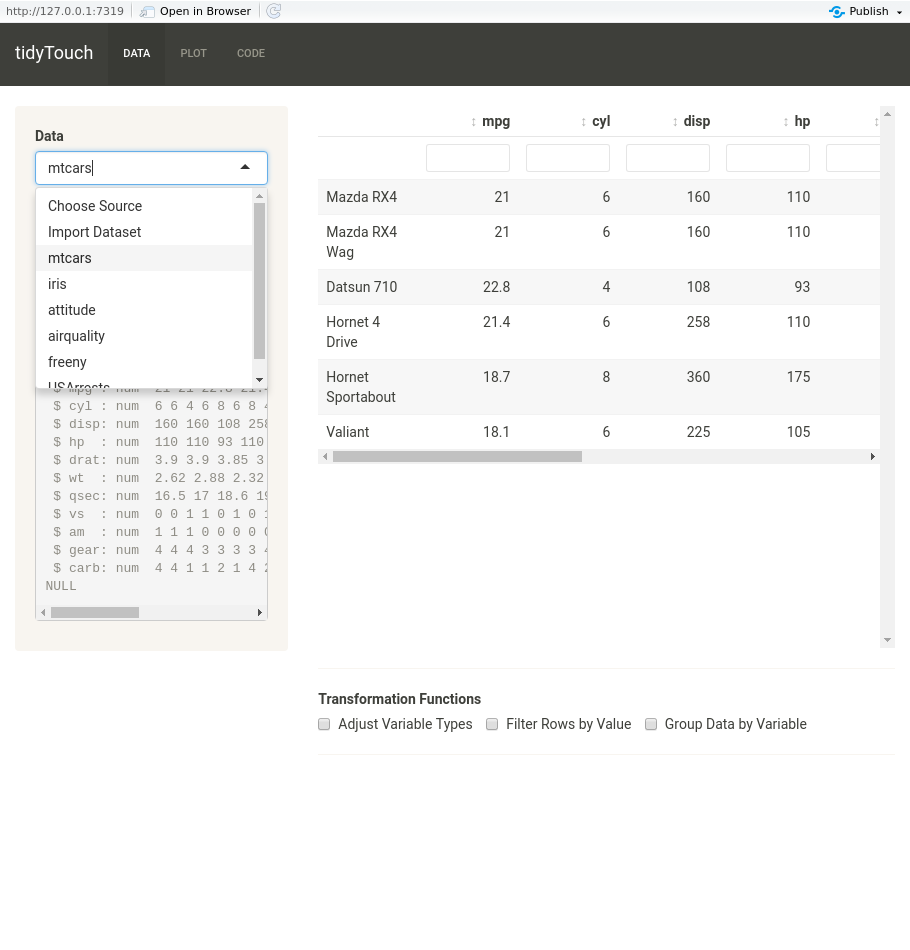
\includegraphics{~/tidyTouch/data_source.png}
\newpage
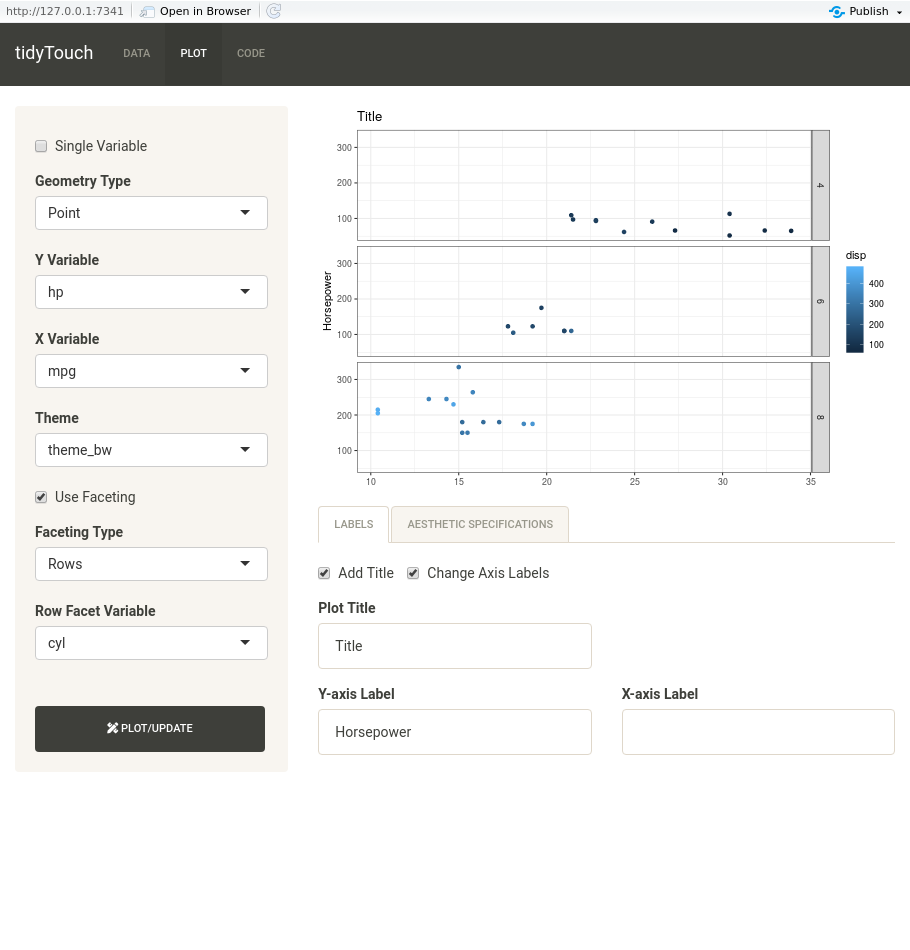
\includegraphics{~/tidyTouch/plot.png}

\newpage

\hypertarget{references}{%
\section{References}\label{references}}

\begingroup
\setlength{\parindent}{-0.5in}
\setlength{\leftskip}{0.5in}

\hypertarget{refs}{}
\leavevmode\hypertarget{ref-R-papaja}{}%
Aust, F., \& Barth, M. (2020). \emph{papaja: Create APA manuscripts with R Markdown}. Retrieved from \url{https://github.com/crsh/papaja}

\leavevmode\hypertarget{ref-cook-graphs}{}%
Chang, W. (2013). \emph{R graphics cookbook}. (M. Loukides \& C. Nash, Eds.). O'Reilly Media, Inc.

\leavevmode\hypertarget{ref-R-shinythemes}{}%
Chang, W. (2018). \emph{Shinythemes: Themes for shiny}. Retrieved from \url{https://CRAN.R-project.org/package=shinythemes}

\leavevmode\hypertarget{ref-R-shiny}{}%
Chang, W., Cheng, J., Allaire, J., Xie, Y., \& McPherson, J. (2019). \emph{Shiny: Web application framework for r}. Retrieved from \url{http://shiny.rstudio.com}

\leavevmode\hypertarget{ref-spss}{}%
IBM. (2017). SPSS, version 25.0. Retrieved from \url{https://www.ibm.com/analytics/spss-statistics-software}

\leavevmode\hypertarget{ref-R-reactable}{}%
Lin, G. (2019). \emph{Reactable: Interactive data tables based on 'react table'}. Retrieved from \url{https://CRAN.R-project.org/package=reactable}

\leavevmode\hypertarget{ref-excel}{}%
Microsoft. (2019). Microsoft excel, version 16.0.12819.37950. Retrieved from \url{https://products.office.com/en-us/excel}

\leavevmode\hypertarget{ref-minitab}{}%
Minitab. (2020). Minitab statistical software, version 19.2020.1. Retrieved from \url{http://www.minitab.com/en-us/products/minitab/}

\leavevmode\hypertarget{ref-datavis1}{}%
Murray, S. (2017). \emph{Interactive data visualization for the web}. (M. Foley, Ed.) (2nd ed.). O'Reailly Media, Inc.

\leavevmode\hypertarget{ref-osd}{}%
Open Source Initiative. (2020). OSI: Open source definition. Retrieved from \url{https://opensource.org/docs/osd}

\leavevmode\hypertarget{ref-bigdata1}{}%
Piccianio, A. G. (2012). The evolution of big data and learning analytics in american higher education. \emph{Journal of Asynchronous Learning Networks}, \emph{16}(3), 9--20.

\leavevmode\hypertarget{ref-R-base}{}%
R Core Team. (2020). \emph{R: A language and environment for statistical computing}. Vienna, Austria: R Foundation for Statistical Computing. Retrieved from \url{https://www.R-project.org/}

\leavevmode\hypertarget{ref-rstudio}{}%
RStudio Team. (2020). \emph{RStudio: Integrated development environment for r}. Boston, MA: RStudio, Inc. Retrieved from \url{http://www.rstudio.com/}

\leavevmode\hypertarget{ref-R-shinymeta}{}%
Sievert, C. (2019). \emph{Shinymeta: Record and expose shiny app logic using metaprogramming}.

\leavevmode\hypertarget{ref-R-ggplot2}{}%
Wickham, H. (2016). \emph{Ggplot2: Elegant graphics for data analysis}. Springer-Verlag New York. Retrieved from \url{https://ggplot2.tidyverse.org}

\leavevmode\hypertarget{ref-tidyverse}{}%
Wickham, H. (2017). \emph{Tidyverse: Easily install and load the 'tidyverse'}. Retrieved from \url{https://CRAN.R-project.org/package=tidyverse}

\leavevmode\hypertarget{ref-R-readxl}{}%
Wickham, H., \& Bryan, J. (2019). \emph{Readxl: Read excel files}. Retrieved from \url{https://CRAN.R-project.org/package=readxl}

\leavevmode\hypertarget{ref-R-dplyr}{}%
Wickham, H., François, R., Henry, L., \& Müller, K. (2020). \emph{Dplyr: A grammar of data manipulation}. Retrieved from \url{https://CRAN.R-project.org/package=dplyr}

\leavevmode\hypertarget{ref-R-tidyr}{}%
Wickham, H., \& Henry, L. (2020). \emph{Tidyr: Tidy messy data}. Retrieved from \url{https://CRAN.R-project.org/package=tidyr}

\leavevmode\hypertarget{ref-R-readr}{}%
Wickham, H., Hester, J., \& Francois, R. (2018). \emph{Readr: Read rectangular text data}. Retrieved from \url{https://CRAN.R-project.org/package=readr}

\leavevmode\hypertarget{ref-R-haven}{}%
Wickham, H., \& Miller, E. (2019). \emph{Haven: Import and export 'spss', 'stata' and 'sas' files}. Retrieved from \url{https://CRAN.R-project.org/package=haven}

\leavevmode\hypertarget{ref-grammar}{}%
Wilkinson, L. (2005). \emph{The grammar of graphics} (2nd ed.). Springer Scinece \& Business Media.

\leavevmode\hypertarget{ref-bigdata2}{}%
Williamson, B. (2017). \emph{Big data in education}. (J. Clark, Ed.). SAGE Publications Inc.

\leavevmode\hypertarget{ref-R-rmarkdown}{}%
Xie, Y., Allaire, J., \& Grolemund, G. (2018). \emph{R markdown: The definitive guide}. Boca Raton, Florida: Chapman; Hall/CRC. Retrieved from \url{https://bookdown.org/yihui/rmarkdown}

\endgroup

\end{document}
